%%%%%% Run at command line, run
%%%%%% xelatex grad-sample.tex 
%%%%%% for a few times to generate the output pdf file
\documentclass[12pt,oneside,openright,a4paper]{explo-english-project}

 \usepackage{polyglossia}
 \usepackage{graphicx}
 \setdefaultlanguage{english}
 \setotherlanguage{thai}
\defaultfontfeatures{Mapping=tex-text,Scale=1.0,LetterSpace=0.0}
\setmainfont[Scale=1.0,LetterSpace=0,WordSpace=1.0,FakeStretch=1.0]{Times New Roman}
\emergencystretch=10pt
%\XeTeXlinebreaklocale "th_TH"	
%\XeTeXlinebreakskip = 0pt plus 1pt
%\setmathfont(Digits)[Scale=1.0,LetterSpace=0,FakeStretch=1.0]{Times New Roman}


%%% Title Page

% First line of title
\def\disstitleone{Project/Indep study title line 1}   
% Second line of title
\def\disstitletwo{Project/Indep title line 2 (optional)}   

% Members
\def\dissauthor{Ms. Pichyapa Khanapattanawong}
\def\dissauthortwo{Mr. Sakolkrit Pengkhum}
\def\dissauthorthree{Mr. Intouch Yuso}
\def\dissauthorfour{Ms. Ruedhaidham Soros}
\def\dissauthorfive{}

% The degree that you're persuing
\def\dissdegree{Bachelor of Engineering} 	% Name of the degree
\def\dissdegreeabrev{B.Eng} 				% Abbreviation of the degree
\def\dissyear{2021}                  		% Year of submission
\def\thaidissyear{2564}               		% Year of submission (B.E.)


%%% Project and independent study committee

\def\dissadvisor{Aye Thant May}  	% Main Teaching Assistant
% \def\disscommitteetwo{}  			% 3rd committee member (no-need)

\def\worktype{Project} 				% Project or Independent study
\def\disscredit{3}   				% 3 credits or 6 credits (no-need)

\def\fieldofstudy{Computer Engineering} 
\def\department{Computer Engineering} 
\def\faculty{Engineering}
 
\def\appendixnames{Appendix} %%% Appendices or Appendix

%%WWWWWWWWWWWWWWWWWWWWWWWWWWWWWWWWWWWWWWWWWWWWWWWWWWWWWWWWWWWWWWWWWWWWWWWWW%%

%%  ******** Do not modify from this part  ********
\def\thaidissadvisor{} % No-Need
%% Leave this empty if you have no co-advisor
\def\thaidisscoadvisor{} % No-Need
\def\thaidissdegree{วิศวกรรมศาสตรบัณฑิต}

% Change the line spacing here...
\linespread{1.15}

%%%%%%%%%%%%%%%%%%%%%%%%%%%%%%%%%%%%%%%%%%%%%%%%%%%%%%%%%%%%%%%%
% End of personal customization.  ******** Do not modify from this part  ********
% to \begin{document} unless you know what you are doing...
%%%%%%%%%%%%%%%%%%%%%%%%%%%%%%%%%%%%%%%%%%%%%%%%%%%%%%%%%%%%%%%%


%%%%%%%%%%%% Dissertation style %%%%%%%%%%%
%\linespread{1.6} % Double-spaced  
%%\oddsidemargin    0.5in
%%\evensidemargin   0.5in
%%%%%%%%%%%%%%%%%%%%%%%%%%%%%%%%%%%%%%%%%%%
%\renewcommand{\subfigtopskip}{10pt}
%\renewcommand{\subfigbottomskip}{-5pt} 
%\renewcommand{\subfigcapskip}{-6pt} %vertical space between caption
%                                    %and figure.
%\renewcommand{\subfigcapmargin}{0pt}

\renewcommand{\topfraction}{0.85}
\renewcommand{\textfraction}{0.1}

\newtheorem{theorem}{Theorem}
\newtheorem{lemma}{Lemma}
\newtheorem{corollary}{Corollary}

\def\QED{\mbox{\rule[0pt]{1.5ex}{1.5ex}}}
\def\proof{\noindent\hspace{2em}{\itshape Proof: }}
\def\endproof{\hspace*{\fill}~\QED\par\endtrivlist\unskip}
%\newenvironment{proof}{{\sc Proof:}}{~\hfill \blacksquare}
%% The hyperref package redefines the \appendix. This one 
%% is from the dissertation.cls
%\def\appendix#1{\iffirstappendix \appendixcover \firstappendixfalse \fi \chapter{#1}}
%\renewcommand{\arraystretch}{0.8}
%%%%%%%%%%%%%%%%%%%%%%%%%%%%%%%%%%%%%%%%%%%%%%%%%%%%%%%%%%%%%%%%
%%%%%%%%%%%%%%%%%%%%%%%%%%%%%%%%%%%%%%%%%%%%%%%%%%%%%%%%%%%%%%%%


\begin{document}
\pdfstringdefDisableCommands{%
\let\MakeUppercase\relax
}
\begin{center}
  
\includegraphics[width=2.8cm]{./assets/unilogo.jpg}
\end{center}
\vspace*{-1cm}

\maketitlepage
%\makesignaturepage 

% abstract page
%%WWWWWWWWWWWWWWWWWWWWWWWWWWWWWWWWWWWWWWWWWWWWWWWWWWWWWWWWWWWWWWWWWWWWWWWWW%%
%%%%%%%%%%%%%%%%%%%%%%%%%%%%%%%%%%%%%%%%%%%%%%%%%%%%%%%%%%%%%%
%%%%%%%%%%%%%%%%%%%%%%         English abstract         %%%%%%%%%%%%%%%%%%%%%%%
%%%%%%%%%%%%%%%%%%%%%%%%%%%%%%%%%%%%%%%%%%%%%%%%%%%%%%%%%%%%%%
%%WWWWWWWWWWWWWWWWWWWWWWWWWWWWWWWWWWWWWWWWWWWWWWWWWWWWWWWWWWWWWWWWWWWWWWWWW%%
\abstract

In a multihop ad hoc network, the interference among nodes is
  reduced to maximize the throughput by using a smallest transmission
  range that still preserve the network connectivity. However, most
  existing works on transmission range control focus on the
  connectivity but lack of results on the throughput performance. This
  paper analyzes the per-node saturated throughput of an IEEE 802.11b
  multihop ad hoc network with a uniform transmission range. Compared
  to simulation, our model can accurately predict the per-node
  throughput.  The results show that the maximum achievable per-node
  throughput can be as low as 11\% of the channel capacity in a normal
  set of $\alpha$ operating parameters independent of node density. However, if
  the network connectivity is considered, the obtainable throughput
  will reduce by as many as 43\% of the maximum throughput. YOOO

\begin{flushleft}
\begin{tabular*}{\textwidth}{@{}lp{0.8\textwidth}}
\textbf{Keywords}: & Multihop ad hoc networks / Topology control / Single-Hop Throughput
\end{tabular*}
\end{flushleft}
\endabstract

% acknowledgements
% Acknowledgements

\preface
Acknowledge your advisors and thanks your friends here..

% table of contents (autogen)
\tableofcontents   

% list of tables (autogen)
\listoftables

% list of figures (autogen)
\listoffigures                      

% list of symbols
% List of symbols 

\listofsymbols
\begin{flushleft}
\begin{tabular}{@{}p{0.07\textwidth}p{0.7\textwidth}p{0.1\textwidth}}
\textbf{SYMBOL}  & & \textbf{UNIT} \\[0.2cm]
$\alpha$ & Test variable\hfill & m$^2$ \\
$\lambda$ & Interarival rate\hfill &  jobs/second\\
$\mu$ & Service rate\hfill & jobs/second\\
\end{tabular}
\end{flushleft}

% list of vocabulary
\include{./chapters/preface/ListVocabs}

%\setlength{\parskip}{1.2mm}



%%%%% Main Body %%%%%

%%% Chapter 1 - Introduction

\chapter{Introduction}

% Sections in introduction

\section{Background} 
% put the content here

This is the background of the project.

% example for pictures
% \begin{figure}[!h]
% \centering
% 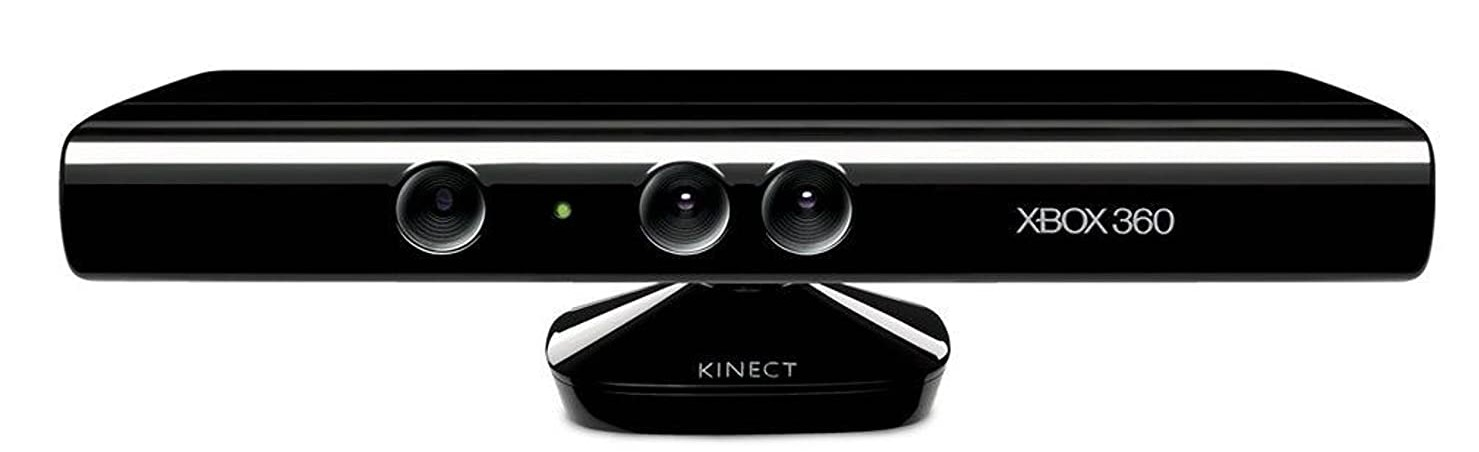
\includegraphics[width=90mm]{X11.jpg}
% \caption{This is the figure Kinect Xbox}\label{fig:x1}
% \end{figure}


\section{Motivations}
% Put the content here
This is our motivations.

% Example for unordered list
\begin{itemize}
\item   What are the problems you are addressing? 
\item  Why they are important?
\item  What are the limitations of existing approaches? 
\end{itemize}
You may combine this section with the background section.

\section{Problem Statements}
% Put content here
This is our problem statement.

\section{Objectives}
% Put content here
This is our objectives.

\section{Scope of Work}
% Put content here
This is our scope.

\section{Project Schedule}
% Put content here

This is our schedule


%%% Chapter 2 - Background Theory and Related work

\chapter{Background Theory and Related Work}

% Resoources urls
\url{http://www.cpe.kmutt.ac.th}
Explain theory, algorithms, protocols, or existing research works and tools related to your work. \cite{santi05b} \cite{bworld,hypersense}

% Create sections and input content files related to background here
\section{Section Name}
% input{./chapters/theory/...}

% Algorithms, related work, development tools

% Example table
% \begin{table}[!h]
% \caption{test table method1}\label{tbl:method1}
% \begin{tabular}{c|c|l|rr} \hline\hline
% Center & Center & left aligned & Right & Right aligned \\ \hline\hline
% Center & Center & left aligned & Right & Right aligned \\ \hline
% \end{tabular}
% \end{table}

% \subsection{Algorithm I}

% Example picture
% \begin{figure}[!h]\centering
% \setlength{\fboxrule}{0.2mm} % can define this in the preamble
% \setlength{\fboxsep}{1cm}
% \fbox{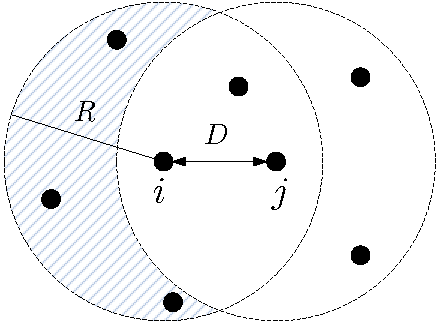
\includegraphics[width=5cm]{./model2.pdf}}
% \caption{The network model}\label{fig:model2}
% \end{figure}


%%% Chapter 3 - Proposed Work

\chapter{Proposed Work}

% Sections in Proposed Work

\section{Graphic Designs}
% put content here
% Character design, map design
% /subsection{}
This is graphic design

\section{Puzzle Design}
% Put content here
% Puzzle questions, puzzle mechanics

This is puzzle design

\section{UXUI Design}
% Put content here
% UXUI Design, User interface,...

This is uxui design

\section{Game Story}
% Put content here
% Game story

This is the game story

\section{Music Design}
% Put content here
% Music Design

This is music design

\section{Dialogue and Interaction}
% Put content here
% dialogue, npc interaction, effects to ending, stat

This is the interactions


%% Chapter 4 - Implementation and results
% implementation / experimental results

\chapter{Implementation Results}

% put content here

% if you want sections
% \section{}
% \input{./chapters/implement/...}


%%% Chapter 5 - Conclusion

\chapter{Conclusions}

\section{Problems and Solutions}
% Problems and solutions

State problems and how you fixed them

\section{Future Works}
% Future Work
What could be done in the future to make your projects better.


%%%%% End of Main body %%%%%


%%% Bibliography
%%%% Comment this in your report to show only references you have
%%%% cited. Otherwise, all the references below will be shown.
%\nocite{*}
%% Use the kmutt.bst for bibtex bibliography style 
%% You must have cpe.bib and string.bib in your current directory.
%% You may go to file .bbl to manually edit the bib items.

\makeatletter
\g@addto@macro{\UrlBreaks}{\UrlOrds}
\makeatother

\bibliographystyle{kmutt}
\bibliography{string,cpe}


%%% Appendices

\appendix{First appendix title}
\noindent{\large\bf Put appropriate topic here} 

% Put content here		% First Appendix
\appendix{Second appendix title}
\noindent{\large\bf Put appropriate topic here} \\

Next, we show how $\mathrm{Var}\{X_n\}$ can be determined.  Let
$C_{\lambda}(l)$ be the autocovariance function of $\lambda_n$.  The
MVA technique basically approximates the input process $\lambda_n$
with a Gaussian process, which allows $\mathrm{Var}\{X_n\}$ to be
represented by the autocovariance function.  In particular, the
variance of $X_n$ can be expressed in terms of $C_{\lambda}(l)$ as
\begin{equation}
  \mathrm{Var}\{X_n\} = nC_{\lambda}(0) + 2\sum_{l=1}^{n-1} (n-l)C_{\lambda}(l)
\end{equation} 

\noindent{\large\bf Add more topic as you need} \\

Therefore, $C_{\lambda}(l)$ must be known in the MVA technique, either
by assuming specific traffic models or by off-line analysis in case of
traces.  In most practical situations, $C_{\lambda}(l)$ will not be
known in advance, and an on-line measurement algorithm developed
in~\cite{eun01} is required to jointly determine both $n^\ast$ and
$m_x$. For fGn traffic, $\mathrm{Var}\{X_n\}$ is equal to $\sigma^2
n^{2H}$, where $\sigma^2 = \mathrm{Var}\{\lambda_n\}$, and we can find
the $n^\ast$ that minimizes (\ref{eq:mx}) directly. Although $\lambda$
can be easily measured, it is not the case for $\sigma^2$ and $H$.
Consequently, the MVA technique suffers from the need of prior
knowledge traffic parameters. 		% Second Appendix

\end{document}
